\chapter{Modelo de Seguridad de Android}
Android \cite{aos} es un sistema operativo de código abierto \cite{aosp}, diseñado para dispositivos móviles y
desarrollado por Google junto con la Open Handset Alliance \cite{oha}. Su arquitectura sigue el estilo arquitectónico conocido como Sistemas Estratificados: los distintos componentes se agrupan en capas según su nivel de abstracción, conformando una jerarquía. Las capas inferiores contienen componentes ligados al \textit{hardware}, mientras que las capas superiores agrupan componentes ligados con tareas de mas alto nivel.\\
Una de las características principales de Android es que cualquier aplicación, ya sea principal o
creada por algún desarrollador, puede, al instalarse con las autorizaciones adecuadas, utilizar tanto
los recursos/servicios del dispositivo móvil como los ofrecidos por el resto de las aplicaciones
instaladas.\\
A lo largo de este capitulo se hará una descripción de los principales aspectos del modelo de seguridad de Android,  en la version 6.0 llamada Marshmallow, lanzada en 2015.
\section{Entorno aislado para cada aplicación}\label{ch01-sandbox}
Fue una de las primeras tecnologías de seguridad aplicadas en Android, y tiene mucha importancia en el modelo de seguridad. Consiste en que cada aplicación se ejecuta en un \emph{entorno aislado}\footnote{Traducción propuesta para el término \textit{sandbox}.}, forzando a que solo pueda tener acceso irrestricto a sus propios recursos. Por lo tanto, las aplicaciones no pueden interactuar entre ellas y tienen acceso limitado al sistema operativo. Cada aplicación se le asigna una única id de usuario UID y se ejecuta en ese usuario como un proceso independiente, tal como se observa en la Figura \ref{fig:ch01:sandbox}.\\
Dado que el \emph{entorno aislado} es a nivel del \textit{kernel}, este modelo de seguridad se extiende al código nativo y a las aplicaciones del sistema operativo, tales como las bibliotecas del sistema operativo y los \textit{frameworks} de las aplicaciones. Esto genera un aislamiento a nivel del \textit{kernel}, ya que todas las políticas que se aplican a usuarios o grupos de usuarios, se transfieren a las aplicaciones por tener su UID.
\begin{figure}[hbtp]
	\begin{center}
		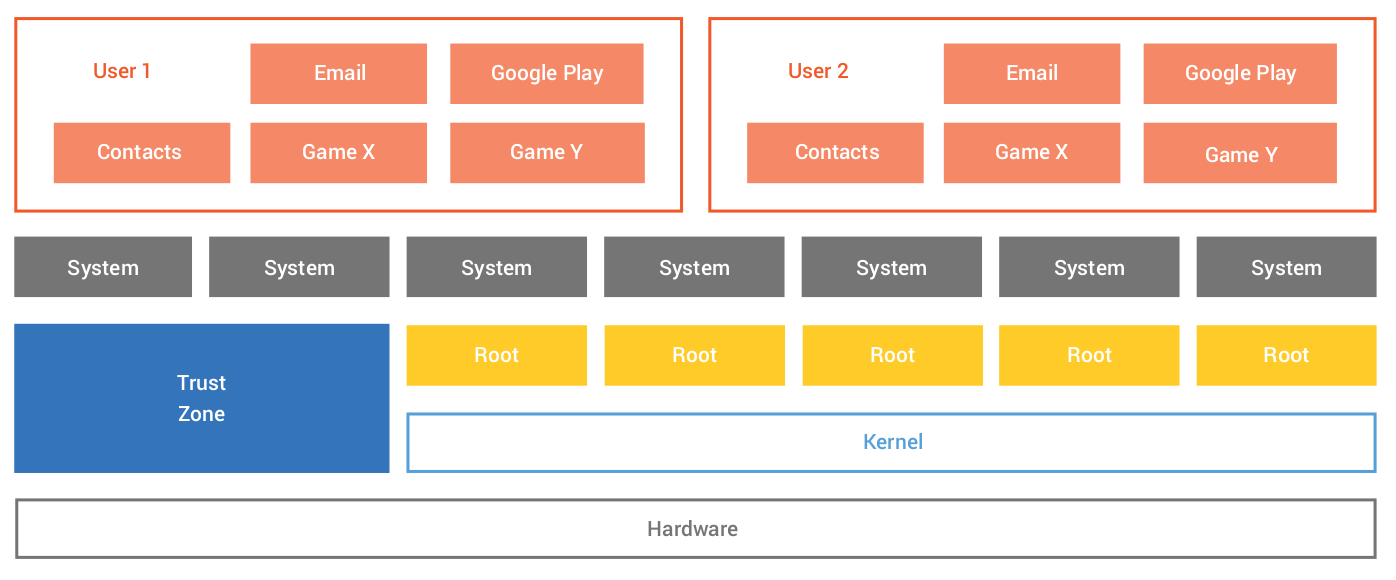
\includegraphics[width=0.75\linewidth]{chapter1/android_security_model}
	    \caption{Aislamiento de las aplicaciones según su UID \cite{asreview2015}.}
	    \label{fig:ch01:sandbox}
    \end{center}
\end{figure}
\section{Políticas de acceso mejoradas}
\emph{SELinux}\footnote{\textit{Security Enhanced Linux}, por sus siglas en inglés.} es un sistema de políticas de acceso obligatorio para Linux. Por lo tanto, siempre se consulta a una autoridad central para permitir cualquier acceso a un recurso; abarca a todos los procesos, inclusive aquellos que corren con privilegios de \textit{root}. \emph{SELinux} opera bajo \textit{the ethos of default denial}, es decir, todo lo que no está explícitamente permitido es denegado. Puede trabajar en dos modos:
\begin{itemize}
    \item \underline{Riguroso:} aplica estrictamente las políticas de seguridad.
    \item \underline{Permisivo:} no se aplican las políticas pero se guardan en un log.
\end{itemize} 
Decimos que un dominio es una etiqueta que identifica un conjunto de procesos en una política de seguridad. Los procesos que comparten una misma etiqueta de dominio son tratados de la misma forma. \\
Android permite aplicar el modo permisivo en un determinado dominio y el resto del sistema permanece en modo riguroso. Gracias a ello, se puede lograr aplicar incrementalmente \emph{SELinux} a una porción cada vez mayor del sistema y desarrollar de políticas para nuevos servicios, manteniendo el resto del sistema en vigencia.
\section{Autenticación del usuario}
Android provee diversas formas para que un usuario se autentique, con el objetivo de desbloquear la pantalla. Desde los comienzos, la autenticación se realizaba mediante el PIN, contraseña y patrones. A partir de la versión 5.0, se introduce el concepto llamado \textit{TrustAgents}, el cuál permite mecanismos de desbloqueo más flexibles, tales como:
\begin{itemize}
	\item Reconocimiento facial.
	\item Un determinado lugar, configurado a través de Google Maps.
	\item Reconocimiento de voz.
	\item Ciertos dispositivos, tales como el auto (a través de Bluetooth).
\end{itemize}
La novedad en la versión 6.0 es que soporta el lector de huellas digitales.\\
Dependiendo del método utilizado para autenticarse, el sistema operativo provee dos componentes: \textit{Gatekeeper} y \textit{Fingerprint}. El primer componente realiza la autenticación del patrón/contraseña del dispositivo en un entorno de ejecución de confianza TEE); mientras que el segundo componente es el encargado de verificar que la huella detectada por el sensor es valida. Ellos interactúan con el \textit{Keystore}\footnote{Es un componente para almacenar las claves criptográficas, el cual dificulta su extracción, ya que asegura dos cosas: una clave nunca entra en una aplicación y una clave nunca sale de una zona segura \cite{dakss}.} para soportar el uso de \textit{tokens} de autenticación respaldados por \textit{hardware} (\textit{AuthTokens}).\\
La verificación del desbloqueo de la pantalla ocurre en el TEE \footnote{El \textit{Trust Execution Enviroment} es una zona segura del procesador principal en la cual se provee una ejecución segura e íntegra, tanto de código fuente como de datos. El TEE aisla por \textit{hardware} el acceso a cierta memoria y provee mecanismos de I/O para dicha memoria \cite{tee2011}.}, tal como se observa en la Figura \ref{fig:ch01:authentication-flow}.
\begin{figure}[htbp]
	\begin{center}
		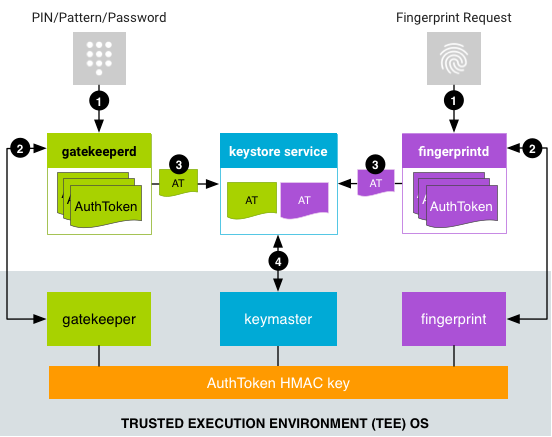
\includegraphics[width=0.7\linewidth]{chapter1/authentication-flow}
		\caption{Proceso de autenticación en Android\cite{aossec}.}
		\label{fig:ch01:authentication-flow}
	\end{center}
\end{figure}
Como consecuencia del esta forma de autenticarse, se destacan las siguientes ventajas:
\begin{itemize}
    \item Al permitir el desbloqueo con datos biométricos, se acelera y se simplifica el proceso de autenticación. Los usuarios eligen este sistema de desbloqueo en un 91\% \cite{asreview2015}.
    \item Al realizarse la autenticación en un TEE, se mejora la protección contra ataques de fuerza bruta, ya que se incrementa exponencialmente el tiempo de espera para el desbloqueo \cite{asreview2015}.
\end{itemize}
Estas mejoras permiten que los desarrolladores de aplicaciones tengan más opciones de seguridad para sus datos y sus comunicaciones.
\section{Seguridad en las aplicaciones}
\subsection{Permisos} \label{ch01-permisos}
Ciertos recursos que provee Android son sensibles, ya que acceden a datos personales o periféricos importantes. Dichos recursos sólo pueden ser accedidos mediante una SS-API\footnote{\textit{Security Sensitive API}, por sus siglas en inglés.} con un doble objetivo: tenerlos aislados y permitir cierta granularidad de seguridad sobre ellos \cite{HYGZD2014}.
El mecanismo de seguridad para el acceso a estas SS-API de recursos se llama Permisos y se clasifican de acuerdo con el riesgo implícito al otorgarlos en las siguientes cuatro categorías:
\begin{itemize}
    \item \emph{Normal:} Son aquellos permisos de bajo riesgo ya que corresponden a características aisladas y son considerados de bajo riesgo para las demás aplicaciones, para el sistema y para el usuario. Son concedidos automáticamente por el sistema, sin solicitar aprobación explícita del usuario \cite{Rom14}.
    \item \emph{Dangerous:} Son aquellos permisos de alto riesgo ya que resguardan los accesos a información sensible para el usuario u otorgan control sobre funcionalidades principales del sistema. Para ser concedidos se requiere aprobación explícita del usuario \cite{Rom14}. 
    \item \emph{Signature:} Son aquellos permisos que son aprobados solamente si la aplicación que los requiere tiene el mismo certificado que la aplicación que los creó. Cuando el sistema valida el certificado, se otorga el permiso sin requerir aprobación explícita del usuario. Se crearon para permitir que un desarrollador pueda compartir información entre sus distintas aplicaciones sin necesidad de la aprobación del usuario \cite{Rom14}.
    \item \emph{Signature/System:} Son aquellos permisos que controlan el acceso a servicios críticos del sistema. En general, las únicas aplicaciones que los utilizan son las que vienen pre-instaladas en el dispositivo, ya que se utilizan para ciertas situaciones especiales en las que varios proveedores tienen aplicaciones integradas en una imagen del sistema que necesitan compartir funciones específicas explícitamente porque se están creando juntas \cite{Rom14}.
\end{itemize}
\begin{figure}[hbtp]
	\begin{center}
		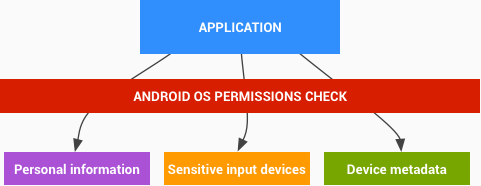
\includegraphics[width=.8\linewidth]{chapter1/permissions_check}
		\caption{Los recursos solamente pueden ser accedidos a través de los permisos}
		\label{fig:ch01:permissions-check}
	\end{center}
\end{figure}
\subsection{Manifiesto}
El archivo de manifiesto proporciona información sobre una aplicación al sistema Android, información que el sistema debe tener para poder ejecutar el código de la aplicación. Es por ello, que todas las aplicaciones deben tener un archivo \texttt{AndroidManifest.xml} (con ese nombre exacto) en el directorio raíz. En este archivo se declaran todos los componentes que forman parte de la aplicación en cuestión, los permisos que son requeridos (ver sección \ref{ch01-permisos}) y los permisos exportados por la aplicación, entre otras cosas.
\begin{figure}[hbtp]
    \centering
    \lstinputlisting[language=XML, basicstyle=\tiny, breaklines=true, frame=single]{AndroidManifest.xml}
    \caption{Manifiesto de la aplicación que contiene los tests.}
    \label{fig:ch01:manifest}
\end{figure}